% $HeadURL$

\paragraph{Glyph: \glyph{Empty Set}}
\label{sec:sourceSink}

It is useful to have the ability to represent the creation of an entity or
a state from an unspecified source, that is, from something that one does
not need or wish to make precise.  For instance, in a model where the
production of a protein is represented, it may not be desirable to
represent all of the amino acids, sugars and other metabolites used, or the
energy involved in the protein's creation.  Similarly, we may not wish to
bother representing the details of the destruction or decomposition of some
biochemical species into a large number of more primitive entities,
preferring instead to simply say that the species ``disappears into a
sink''.  Yet another example is that one may need to represent an input
(respectively, output) into (resp. from) a compartment without explicitly
representing a transport process from a source (resp. to a target).

For these and other situations, SBGN defines a single glyph to handle
these situations representing the involvement of an external pool of entities.  The symbol
used in SBGN is borrowed from the mathematical symbol for ``empty set'',
but it is important to note that it does not actually represent a true
absence of everything or a physical void---it represents the absence of the
corresponding structures in the model, that is, the fact that the
external pool is conceptually outside the scope of the map.

A frequently asked question is, why bother having an explicit symbol at
all?  The reason is that one cannot simply use an arc that does not
terminate on a node, because the dangling end could be mistaken to be
pointing to another node in the map.  This is specially true if the
map is rescaled, causing the spacing of elements in the map to
change.  The availability and use of an explicit symbol for sources and
sinks is critical.

\begin{glyphDescription}

\item[Identifying Attributes:]\mbox{} All glyphs represent the same
  pool of external entities.

\item[Special constraints or rules:]\mbox{}\newline None.

\glyphSboTerm SBO:0000291 ! empty set

\glyphContainer Represented by the mathematical symbol for ``empty
set'', that is, a circle crossed by a bar linking the upper-right and
lower-left corners of an invisible square drawn around the circle ($\emptyset$).
\fig{sourceSink} illustrates this.  The symbol should be linked to one
and only one edge in a map.

\glyphLabel None

\glyphAux None

\glyphCloning All glyphs are identical and therefore clones. No
special decoration is used to indicate this.

\end{glyphDescription}

\begin{figure}[H]
  \centering
  \includegraphics[scale = 0.3]{images/sourceSink}
  \caption{The \glyph{empty set} glyph.}
  \label{fig:sourceSink}
\end{figure}






% The following is for [X]Emacs users.    Please leave in place.
% Local Variables:
% TeX-master: "../sbgn_PD-level1"
% End:
